\documentclass{beamer}
\usetheme{COURS}
\usepackage{tcolorbox}
\usepackage{textpos}
\usetikzlibrary{arrows,automata}


\def\red{\color{red}}
\def\blue{\color{blue}}
\def\green{\color{green}}

\def\opstyle#1{\ensuremath{\operatorname{#1}}}

\title[Codes de Gray combinatoires]%
{\bf Codes de Gray}
\author{\textbf{\Large Florent Hivert}\\[5mm]
  Mél : \texttt{Florent.Hivert@lri.fr}\\
  Adresse universelle : \texttt{http://www.lri.fr/\~{ }hivert}
}
\date{}

\begin{document}
\newcommand{\Count}{\opstyle{count}}
\newcommand{\List}{\opstyle{list}}
\newcommand{\Iter}{\opstyle{iter}}
\newcommand{\Unrank}{\opstyle{unrank}}
\newcommand{\Rank}{\opstyle{rank}}
\newcommand{\First}{\opstyle{first}}
\newcommand{\Next}{\opstyle{next}}
\newcommand{\Random}{\opstyle{random}}

\newcommand{\Concat}{\opstyle{concat}}
\newcommand{\BS}{\opstyle{BitString}}
\newcommand{\Perm}{\opstyle{Perm}}
\newcommand{\Union}{\opstyle{Union}}
\newcommand{\Prod}{\opstyle{Prod}}

\newcommand{\Pos}{\opstyle{Pos}}
\newcommand{\Bin}{\opstyle{Bin}}
\newcommand{\Gray}{\opstyle{Gray}}

\newcommand{\mA}{\mathcal{A}}
\newcommand{\mB}{\mathcal{B}}
\newcommand{\mC}{\mathcal{C}}
\newcommand{\mD}{\mathcal{D}}
\newcommand{\mE}{\mathcal{E}}
\newcommand{\mI}{\mathcal{I}}
\newcommand{\mZ}{\mathcal{Z}}

\newcommand{\Oh}{O}

%***********************************************************************
\frame{\titlepage}
%***********************************************************************
\begin{frame}{Objectifs : Complexité optimale pour $\Iter$}

  L'ordre lexicographique est pratique pour faire de la génération
  combinatoire, \textbf{mais ...}
  \bigskip

  \begin{NOTE}
    Les algorithmes d'itérations vue en cours sont pour la plupart en {\red
      temps constant amorti} (CAT). On peut trouver des algoritmes réellement
    en {\green temps constant} ! Pour ceci, il faut \textbf{changer l'ordre
      d'énumération}.
  \end{NOTE}
\end{frame}

\begin{frame}{Exemple: les chaines de bits}

  \begin{itemize}
  \item Soit $B_n$ le nombre de bits écrit lors de l'itéreration le long de la
    liste lexicographique des mots binaires de longueurs $n$.
  \[B_0 = 0,\qquad B_1=2,\qquad B_{n} = 2B_{n-1}+2\]
  \bigskip\pause

  \item On trouve : $B_n = 2^{n+1} - 2$ pour $2^n$ chaîne de bits.
  \bigskip\pause

  \item En moyenne $\frac{2^{n+1} - 2}{2^n}\approx 2$~bits par itération.
  \end{itemize}
\end{frame}

\begin{frame}{Algorithme en temps constant !}

  \begin{NOTE}
    Il existe des algorithmes en temps constant (non amorti) ! Ce sont des
    algorithmes très simple et très cours: pas de boucle !
  \end{NOTE}
  \bigskip\pause

  \begin{problem}
    D'un objet au suivant, on veux changer le minimum de chose.
  \end{problem}
  \bigskip\pause
  Exemple: 1 bits
\end{frame}

\begin{frame}{Code de Gray combinatoire}

  \begin{DEFN}
    Soit $E$ un ensemble à enumérer. Soit $P$ une relation sur $E$, dite de
    \textbf{proximité}. Un code de \emph{code de Gray combinatoire} pour le
    système $(E, P)$ est une liste $S = s_1, s_2, \dots, s_N$, où $N=|E|$, tel
    que chaque élément de $E$ apparaît une fois et une seule dans $S$ et
    $(s_i,s_{i+1})\in P$ pour tout $i = 1,\dots N-1$.
  \end{DEFN}
  \pause\bigskip
  \begin{itemize}
  \item Dans la plupart des cas la relation $P$ est symétrique.
  \pause\medskip
  \item Problème de théorie des graphes (chemin Hamiltonien).
  \pause\medskip
  \item On dit que le code est cyclique si de plus $(S_n, s_0)\in P$.
  \end{itemize}
\end{frame}

\begin{frame}{Les hypercubes}

  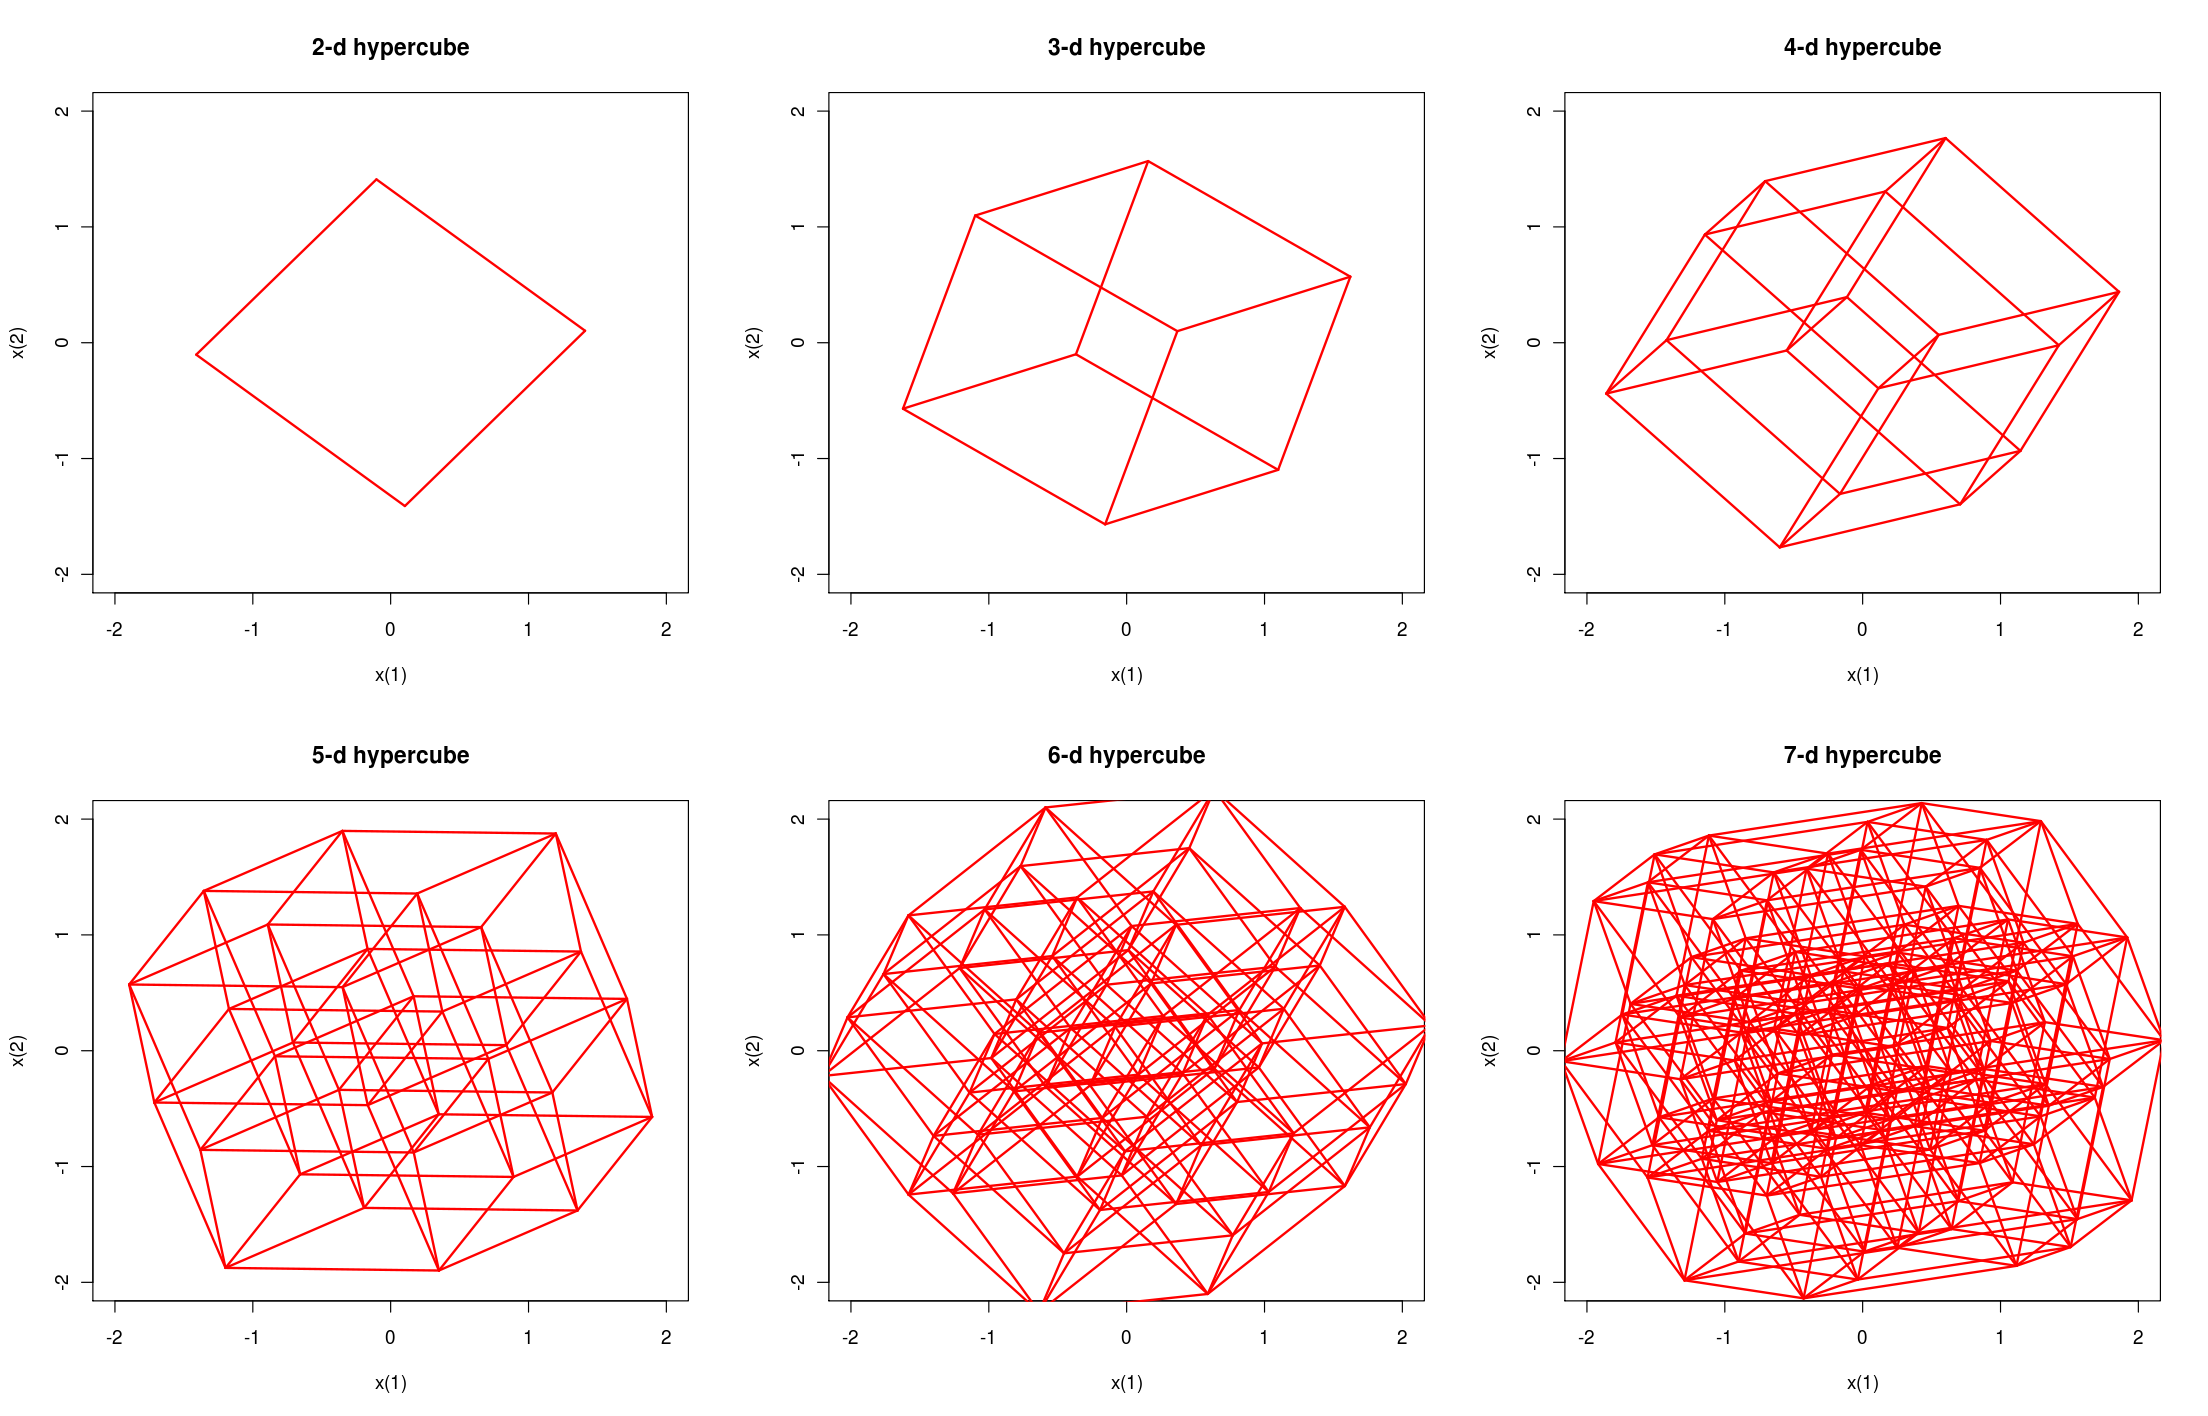
\includegraphics[width=\textwidth]{media/hcube.png}
\end{frame}

\begin{frame}{Code binaire réfléchi}

  Frank Gray 1953
  \bigskip

  \begin{DEFN}
    Idée: on retourne la liste pour la deuxième partie:
    \begin{itemize}
    \item $G_0= [\epsilon]$
    \item $G_n= 0\cdot G_{n-1} + 1\cdot \overline{G_{n-1}}$
    \end{itemize}
  \end{DEFN}
  \[0, 1\]
  \[00, 01, 11, 10\]
  \[000, 001, 011, 010, 110, 111, 101, 100\]
\end{frame}

\begin{frame}{Codage vers le code Gray}

  \begin{NOTE}
    Une formule étonnamment simple
    \[G = i \oplus (i \gg 1)\]
    où $\oplus$ désigne le Ou-Exclusif bit à bit.
  \end{NOTE}
\end{frame}


\begin{frame}{Passage d'une liste de bits à la suivante en temps constant}

Idée: noter la position du prochain zéro:
\begin{NOTE}
  \[ \Pos_i :=
  \begin{cases}
    i & \text{si $b_i=0$ ou $b_{i-1}=1$ } \\
    \min\{k \mid b_k = 0 \text{ et } k > i\} & \text{si $b_i=1$ et $b_{i-1}=0$ } \\
  \end{cases}
  \]
\end{NOTE}
\[\begin{array}{c|cccccccc}
i      &  7 & 6 & 5 & 4 & 3 & 2 & 1 & 0 \\\hline
b_i    &  1 & 0 & 1 & 1 & 1 & 0 & 1 & 0 \\
\Pos_i &  8 & 6 & 5 & 4 & 6 & 2 & 2 & 0 \\
  \end{array}\]
Note: on complète par un $0$ en tête si nécessaire.
\end{frame}

\begin{frame}{Passage d'une liste de bits à la suivante en temps constant}

\begin{NOTE}
  D'un nombre au suivant, au plus trois valeurs du tableau $\Pos$ changent.
\end{NOTE}
\[\begin{array}{ccccc}
n & \Bin & \Pos  &  \Pos_0 & \Gray \\\hline
0 & 000 & 210 & 0 & 000\\
1 & 001 & 211 & 1 & 001\\
2 & 010 & 220 & 0 & 011\\
3 & 011 & 212 & 2 & 010\\
4 & 100 & 310 & 0 & 110\\
5 & 101 & 311 & 1 & 111\\
6 & 110 & 230 & 0 & 101\\
7 & 111 & 213 & 3 & 100\\
\end{array}\]
\end{frame}


\begin{frame}{Exemple: Les permutations}

  \begin{NOTE}{Permutations par transpositions élémentaires}
    \begin{itemize}
    \item $S = $ ensemble des permutations de $[1, 2, \dots, n]$ \bigskip
    \item Relation de proximité: soit $S=(s_1,s_2,\dots s_n)$. Alors $T$ est
      proche de $S$ si on peut trouver $i$ tels que
      \[ T = (s_1, s_2, \dots, s_{i+1}, s_i, \dots s_n)\]
    \end{itemize}
  \end{NOTE}
\end{frame}
\begin{frame}{Le graphe des permutations: le permutohedre}

  \[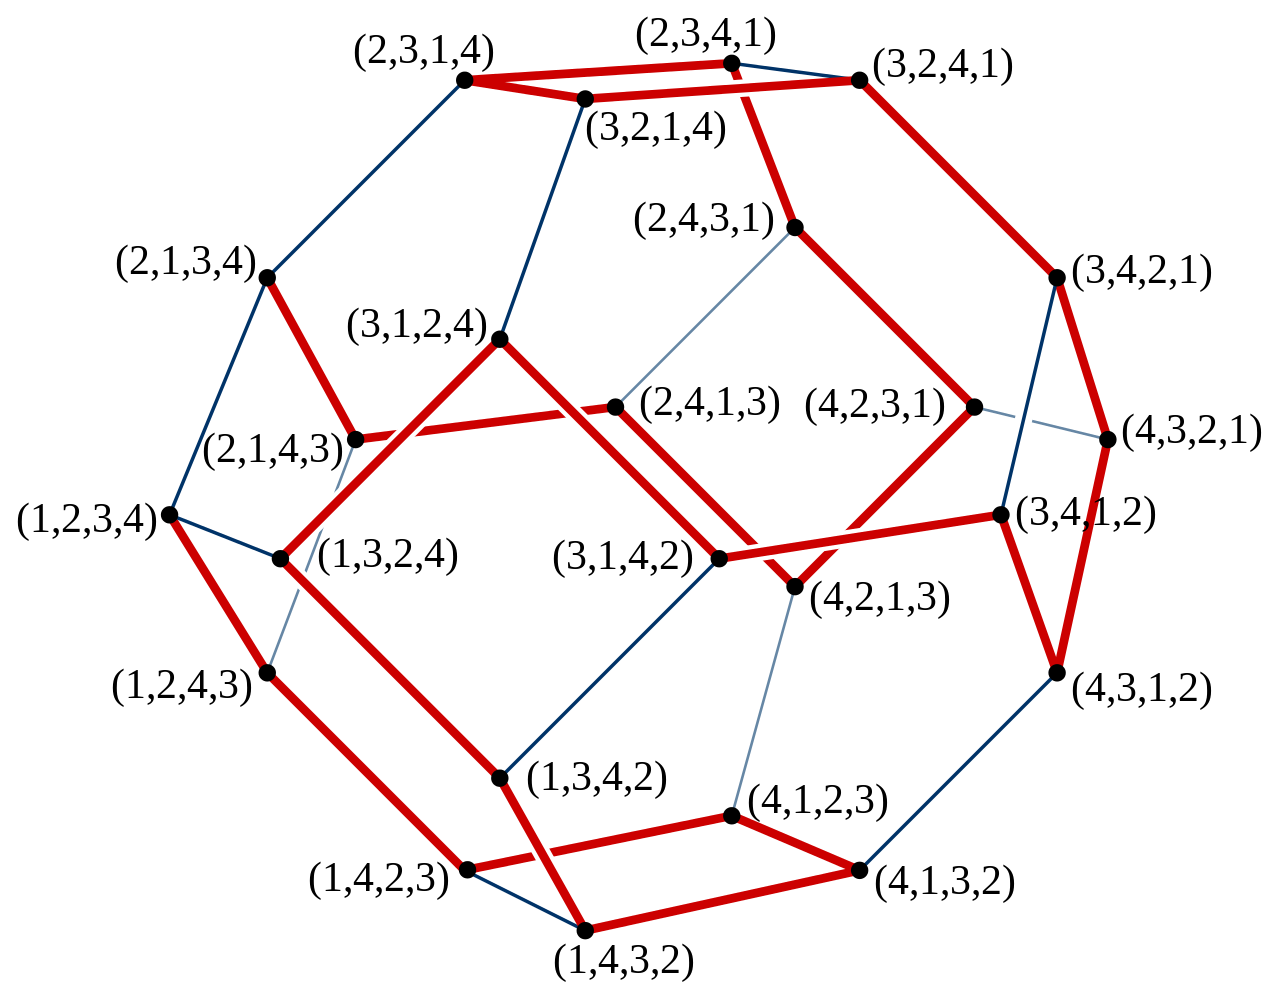
\includegraphics[width=9cm]{media/Steinhaus-Johnson-Trotter-Permutohedron.png}\]
\end{frame}

\begin{frame}{Algorithme de Steinhaus-Johnson-Trotter}

  \begin{NOTE}
    Idée: récursivement insérer $n$ à toute les places possibles en alternant
    le sens de déplacement, d'une permutation à l'autre.
  \end{NOTE}
  \bigskip
  \[\begin{array}{c|c|cccc}
   123 & < & 123{\bf4} & 12{\bf4}3 & 1{\bf4}23 & {\bf4}123 \\
   132 & > & {\bf4}132 & 1{\bf4}32 & 13{\bf4}2 & 132{\bf4} \\
   312 & < & 312{\bf4} & 31{\bf4}2 & 3{\bf4}12 & {\bf4}312 \\
   321 & > & {\bf4}321 & 3{\bf4}21 & 32{\bf4}1 & 321{\bf4} \\
   231 & < & 231{\bf4} & 23{\bf4}1 & 2{\bf4}31 & {\bf4}231 \\
   213 & > & {\bf4}213 & 2{\bf4}13 & 21{\bf4}3 & 213{\bf4} \\
  \end{array}\]
  Voir code Python\dots
\end{frame}
\end{document}
